%%%%%%%%%%%%%%%%%%%%%%%%%%%%%%%%%%%%%%
% LaTeX poster template
% Created by Nathaniel Johnston
% August 2009
% http://www.nathanieljohnston.com/2009/08/latex-poster-template/
%%%%%%%%%%%%%%%%%%%%%%%%%%%%%%%%%%%%%%


\documentclass[final]{beamer}
\usepackage[scale=1.24]{beamerposter}
\usepackage{graphicx}			% allows us to import images
\usepackage{wrapfig}	

\usepackage[utf8]{inputenc}
\usepackage[MeX]{polski}
\usepackage[T1]{fontenc}
\usepackage[english, polish]{babel}


\usepackage{etoolbox,refcount}
\usepackage{multicol}
\usepackage{subfigure}

\newcounter{countitems}
\newcounter{nextitemizecount}
\newcommand{\setupcountitems}{%
  \stepcounter{nextitemizecount}%
  \setcounter{countitems}{0}%
  \preto\item{\stepcounter{countitems}}%
}
\makeatletter
\newcommand{\computecountitems}{%
  \edef\@currentlabel{\number\c@countitems}%
  \label{countitems@\number\numexpr\value{nextitemizecount}-1\relax}%
}
\newcommand{\nextitemizecount}{%
  \getrefnumber{countitems@\number\c@nextitemizecount}%
}
\newcommand{\previtemizecount}{%
  \getrefnumber{countitems@\number\numexpr\value{nextitemizecount}-1\relax}%
}
\makeatother    
\newenvironment{AutoMultiColItemize}{%
\ifnumcomp{\nextitemizecount}{>}{2}{\begin{multicols}{2}}{}%
\setupcountitems\begin{itemize}}%
{\end{itemize}%
\unskip\computecountitems\ifnumcomp{\previtemizecount}{>}{3}{\end{multicols}}{}}

%-----------------------------------------------------------
% Define the column width and poster size
% To set effective sepwid, onecolwid and twocolwid values, first choose how many columns you want and how much separation you want between columns
% The separation I chose is 0.024 and I want 4 columns
% Then set onecolwid to be (1-(4+1)*0.024)/4 = 0.22
% Set twocolwid to be 2*onecolwid + sepwid = 0.464
%-----------------------------------------------------------

\newlength{\sepwid}
\newlength{\onecolwid}
\newlength{\twocolwid}
\newlength{\threecolwid}
\setlength{\paperwidth}{48in}
\setlength{\paperheight}{36in}
\setlength{\sepwid}{0.024\paperwidth}
\setlength{\onecolwid}{0.22\paperwidth}
\setlength{\twocolwid}{0.464\paperwidth}
\setlength{\threecolwid}{0.708\paperwidth}
\setlength{\topmargin}{-0.5in}
\usetheme{confposter}
\usepackage{exscale}

%-----------------------------------------------------------
% The next part fixes a problem with figure numbering. Thanks Nishan!
% When including a figure in your poster, be sure that the commands are typed in the following order:
% \begin{figure}
% \includegraphics[...]{...}
% \caption{...}
% \end{figure}
% That is, put the \caption after the \includegraphics
%-----------------------------------------------------------

\usecaptiontemplate{
\small
\structure{\insertcaptionname~\insertcaptionnumber:}
\insertcaption}

%-----------------------------------------------------------
% Define colours (see beamerthemeconfposter.sty to change these colour definitions)
%-----------------------------------------------------------

\setbeamercolor{block title}{fg=ngreen,bg=white}
\setbeamercolor{block body}{fg=black,bg=white}
\setbeamercolor{block alerted title}{fg=white,bg=dblue!70}
\setbeamercolor{block alerted body}{fg=black,bg=dblue!10}

%-----------------------------------------------------------
% Name and authors of poster/paper/research
%-----------------------------------------------------------

\title{Implementacja aplikacji wspomagającej diagnostykę nowotworu prostaty, wykorzystującej standard DICOM do integracji z realnym systemem szpitalnym}
\author{Rafał Buzun, Łukasz Berwid, Jakub Karolak}
\institute{Politechnika Warszawska, Wydział Matematyki i Nauk Informacyjnych \\
Praca inżynierska}


%-----------------------------------------------------------
% Start the poster itself
%-----------------------------------------------------------

\begin{document}
\begin{frame}[t]
  \begin{columns}[t]												% the [t] option aligns the column's content at the top
    \begin{column}{\sepwid}\end{column}			% empty spacer column
    \begin{column}{\onecolwid}
      \begin{block}{Streszczenie}
      Obecnie prostata liczona jest ze wzoru, który aproksymuje kształt gruczołu elipsoidą. W pracy dyplomowej przedstawiamy alternatywne metody obliczania objętości, mogące znacząco poprawić dokładność obliczeń. \newline 
      Opisany system pozwala na segmentację obrazów gruczołu pochodzącego z obrazowania metodą multiparametrycznego rezonansu magnetycznego oraz obliczanie objętości na podstawie masek segmentacji. Narzędzie zostało przygotowane do integracji ze szpitalnym systemem PACS.  Dodatkowo stworzona została baza badań zawierająca informacje o referencyjnych wartościach objętości gruczołu krokowego pochodzących z estymacji bazującej na obrazowaniu ultrasonografem. 
      \end{block}
      \vskip2ex
      \begin{block}{Wstęp}
Rak prostaty to drugi po raku płuc najczęściej diagnozowany nowotwór u mężczyzn. W ciągu ostatnich lat w Polsce wzrasta zachorowalność na raka stercza, a także – choć w mniejszym stopniu – umieralność. Krajowy rejestr nowotworów zanotował, że w naszym kraju w 2015 r. zostało wykrytych 14 tys. nowych przypadków raka prostaty, a 5 tys. chorych z wcześniej wykrytą chorobą umarło. W 2012 roku, 7 lat temu, z powodu tego nowotworu zachorowało 11 tys. mężczyzn, a 4,1 tys. zmarło. \newline 
Mając na uwadze powyższe statystyki, w niniejszej pracy podjęto się zbadania możliwości automatyzacji wykrywania prostaty na zdjęciach rezonansu magnetycznego, poprzez automatyczną segmentację prostaty i obliczanie objętości. Algorytmy obliczania wielkości gruczołu opisane w tej pracy mogą być wskazówką dla lekarza podczas stawiania diagnozy.
      \end{block}
      \vskip2ex
    \end{column}

    \begin{column}{\sepwid}\end{column}			% empty spacer column
    \begin{column}{\threecolwid}					  % create a three-column-wide column and then we will split it up later
      \begin{block}{Rezultaty}
      \begin{wrapfigure}{r}{30cm}
		\caption{Wykres przedstawiający wyniki}\label{wrap-fig:1}
		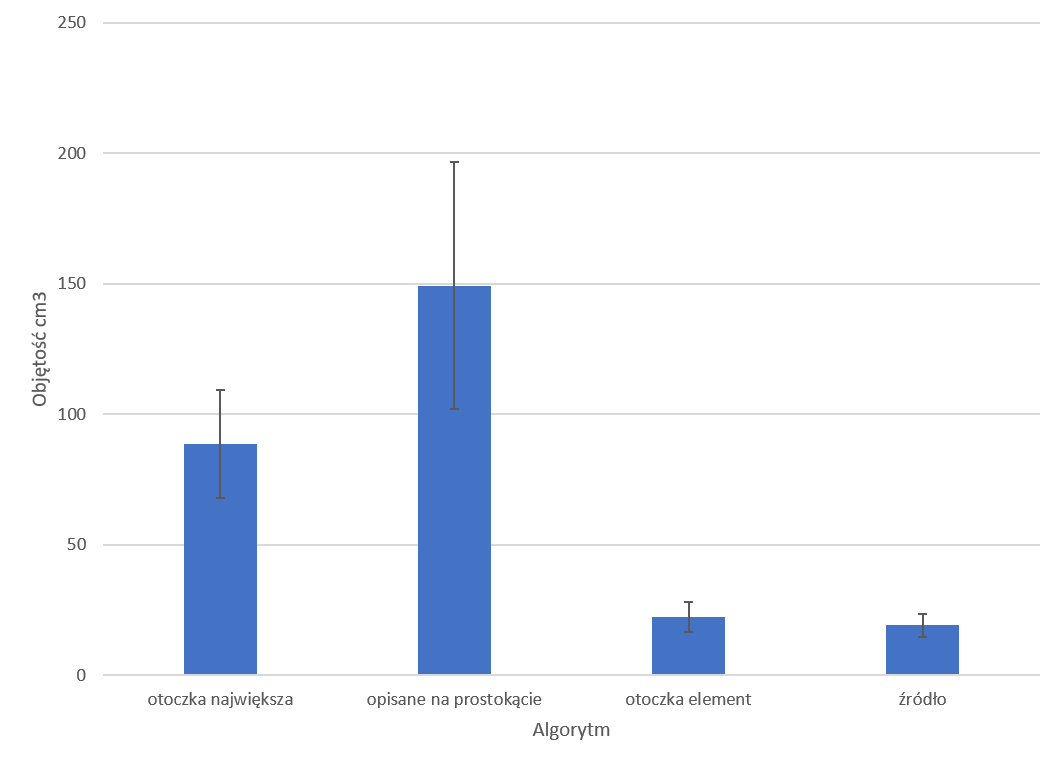
\includegraphics[width=30cm]{WynikiObjetosc.png}
	\end{wrapfigure} 
%------------------------------------------
        Dane wykożystane w pracy zawierały obrazowanie prostat, których średnia objętość wynosiła 19 $cm^3$ oznacza to, że zebrane dane dotyczyły zdrowych gruczołów. \newline Algorytm proponowany przez nas, który osiągnął najlepszy wynik to metoda liczenia otoczki wypukłej wokół największego spójnego elementu maski. Osiągnął on średni wynik 22 $cm^3$, czyli odbiega od wartości oczekiwanej tylko o 3 $cm^3$. \newline
         Jest to znacząca poprawa względem metody aproksymowania elipsoidą, która dawała średni wynik na poziomie 53 $cm^3$ na danych testowych. Na podstawie zebranych danych ilościowych ze szpitala średnia objętość prostaty na podstawie wymiarów z MRI średnia objętość to 50 $cm^3$. \newline 
         Jednak ze względu na wiek pacjentów, u których występuje podejrzenie obecności nowotworu prostaty częstym schorzeniem jest rozrost prostaty. To wpływa na jej zmienność manifestowaną również w wynikach obrazowania MRI. Zmieniona anatomia w przypadku pacjentów z podejrzeniem raka prostaty poddaje w wątpliwość dokładność stosowanie algorytmów sztucznej inteligencji wyuczonych na danych pochodzących ze zdrowych pacjentów.
        \par
Na wykresie ~\ref{wrap-fig:1} przedstawiamy dokładne wyniki każdego z algorytmów.
      \end{block}
      \begin{columns}[t,totalwidth=\threecolwid]	% split up that three-column-wide column
        \begin{column}{\onecolwid}
          \begin{block}{Opis badań}
			Zostało przeprowadzone badanie czy i w jakim stopniu objętości uzyskane poprzez badanie USG oraz MR są skorelowane. Analiza została wykonana na próbce szpitalnej pochodzącej ze szpitala MSWiA zawierającą dane 222 mężczyzn, w wieku między 31 a 87 lat.  
			W danych szczególną uwagę należało zwrócić na: 			
            \begin{AutoMultiColItemize}
                \item wiek pacjenta 
                \item wywiad środowiskowy 
                \item wynik w skali Gleasona
                \item wynik biopsji
                \item PSA
                \item PIRADS 
            \end{AutoMultiColItemize}
			Z przeprowadzonych obliczeń wynika, że te dwie objętości są ze sobą w silnej korelacji. Współczynnik korelacji dla tych dwóch zmiennych wynosi 0.76 (p<0,001).
          	\begin{figure}
				\caption{Korelacja USG i MR}
				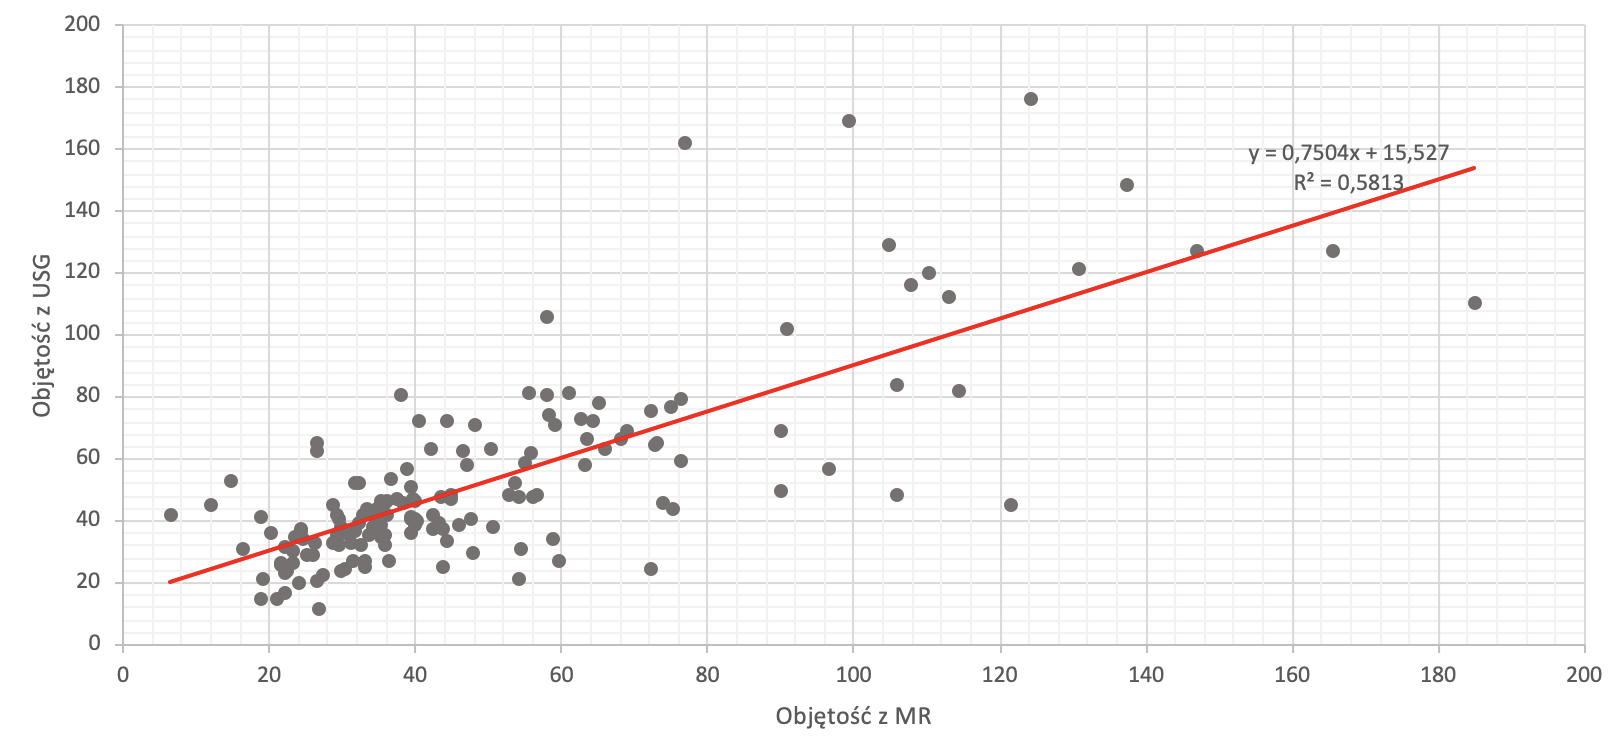
\includegraphics[width=20cm]{Scatter.png}
			\end{figure}
          \end{block}
        \end{column}
        \begin{column}{\onecolwid}
  			\begin{block}{Segmentacja}
			Do segmentacji prostaty został użyty algorytm oparty o uproszczoną sieć U-Net. Rozwiązanie zostało wybrane, ponieważ sieć jest symetryczna, dzięki czemu zyskujemy większą dokładność znajdowania regionów obrazu oraz pomija kilka warstw co skutkuje lepszymi rezultatami przy małej ilości danych. \newline
			Do wytrenowania sieci zostały użyte dane pochodzące z konkursu \textit{Automated Segmentation of Prostate Structures Challange}. Zawierały 60 pacjentów, łącznie 1073 obrazów. \newline
			Po nauczeniu sieci osiągnęliśmy współczynnik podobieństwa równy około 0.70 na danych testowych.
                \begin{figure}[htb]
                    \centering % <-- added
                    \begin{subfigure}{}
                        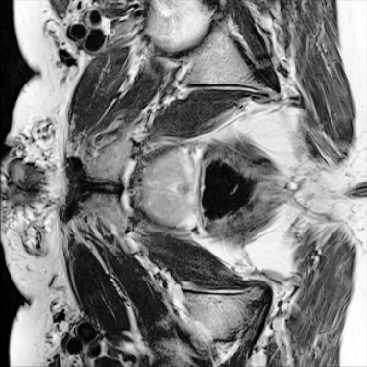
\includegraphics[width=7cm,angle=270,origin=c]{../segmentation/segmentation_train_1.png}
                        \label{fig:1}
                    \end{subfigure}\hfil % <-- added
                    \begin{subfigure}{}
                        
\includegraphics[width=7cm,angle=270,origin=c]{../segmentation/segmentaion_mask_1.png}
                        \label{fig:2}
                    \end{subfigure}\hfil % <-- added
                    \begin{subfigure}{}
                        
\includegraphics[width=7cm,angle=270,origin=c]{../segmentation/pred_mask_1.png}
                        \label{fig:3}
                    \end{subfigure}
                    
                    \medskip
                    \begin{subfigure}{}
                        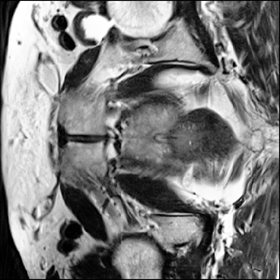
\includegraphics[width=7cm,angle=270,origin=c]{../segmentation/segmentation_train_2.png}
                        \label{fig:4}
                    \end{subfigure}\hfil % <-- added
                    \begin{subfigure}{}
                        
\includegraphics[width=7cm,angle=270,origin=c]{../segmentation/pred_mask_2.png}
                        \label{fig:5}
                    \end{subfigure}\hfil % <-- added
                    \begin{subfigure}{}
                        
\includegraphics[width=7cm,angle=270,origin=c]{../segmentation/segmentation_mask_2.png}
                        \label{fig:6}
                    \end{subfigure}
                    \caption{Przykłady wyników}
                    \label{fig:images}
                \end{figure}
  			\end{block}       
        \end{column}
        \begin{column}{\onecolwid}
          \begin{block}{Technologie wykorzystane w pracy}
			\begin{figure}
				\caption{Schemat architektury aplikacji}
				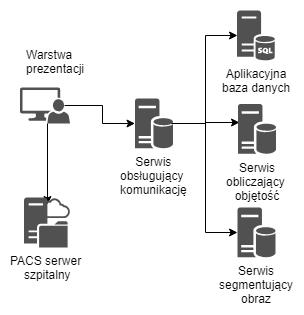
\includegraphics[width=20cm]{Architektura.png}
			\end{figure}
          Aplikacja napisana jest w sposób modularny, każdy z serwisów działa w osobnym kontenerze. Dzięki temu zyskujemy łatwość rozszerzania i wprowadzania kolejnych zmian.
          W aplikacji wykorzystaliśmy technologie
          \begin{AutoMultiColItemize}
          	\item Docker
          	\item .NET Core
          	\item Python
          	\item React.js
  \end{AutoMultiColItemize}
		  \end{block}
        \end{column}
      \end{columns}
      \vskip2.5ex
    \end{column}
  \begin{column}{\sepwid}\end{column}			% empty spacer column
 \end{columns}
\end{frame}
\end{document}
